\chapter{Especificação do Projeto}
\label{Cap:especificacao}

O sistema é composto por duas partes: hardware, ou seja, os componentes como microcontroladores, sensores, entre outros; e software, identificado como o aplicativo de interface entre o usuário e os dados coletados.

O sistema está brevemente descrito através da figura \ref{fig:esqueminha} e a disposição dos componentes através do diagrama de implantação da figura \ref{fig:diagrama_implantacao}:

A parte de hardware está separada em dois módulos principais: o módulo de sensoriamento e um módulo coordenador e a parte de software se resume à parte da aplicação web na nuvem.
\section{Premissas}

Sendo esse um projeto que visa o sensoriamento e de um monitor para vizualisar os dados com o objetivo de dar uma visão geral ao usuário sobre gastos supérfulos e uma relação absoluta do consumo de cada equipamento, o sistema é influenciado por alguns fatores físicos e geopolíticos, o que leva à necessidade de usar algumas premissas que tiveram de ser feitas para ajustar o projeto ao tempo previsto e garantir o funcionamento correto do sistema:

\begin{enumerate}
\item{O usuário deve morar em São Paulo, uma vez que o cálculo da conta de luz é uma função da distribuidora e cada lugar possui uma distribuidora diferente, essa escolha permite minimizar pesquisas de como deve ser calculado a conta em cada região do Brasil}
\item{Será considerado um fator de potência ideal unitário, ou seja, a potência medida no trabalho será a aparente}
\end{enumerate}
\section{Hardware}
\label{Sec:hardware}
\subsection{Módulo Sensor}

O módulo sensor é o responsável por medir e transmitir ao módulo coordenador as informações necessárias para calcular o consumo de energia do equipamento acoplado.

Os componentes físicos do módulo sensor são:

\begin{itemize}
\item Circuito Verificador de tensão
\item Sensor de Corrente (Non-invasive AC Current Sensor)
\item Arduino Uno - R3
\item XBee Shield
\item XBee 2mW PCB Antenna - Series 2
\end{itemize}
%
\subsection{Módulo Coordenador}

O módulo coordenador é o responsável por receber mensagens dos módulos sensores, tratá-los e enviar os dados de consumo para a aplicação em nuvem.

Os componentes do coordenador são:

\begin{itemize}
\item Kit Raspberry Pi2 + Fonte + Microsd 8gb + Wifi Usb
\item XBee Explorer Dongle
\item XBee 2mW PCB Antenna - Series 2
\end{itemize}
%
\subsection{Circuitos}
\subsubsection{Verificador de Tensão}

No circuito de cada módulo de sensor, são feitas detecções da tensão (127V ou 220V) para cálculos de potência.  O objetivo do circuito da figura \ref{fig:voltage-circuit} é indicar se a tensão na tomada é 220V ou 127V. A saída do circuito é usada como um valor analógico, que dependendo da tensão de entrada resultará em faixas diferentes para as diferentes tensões.

\begin{figure}[H]
\centering
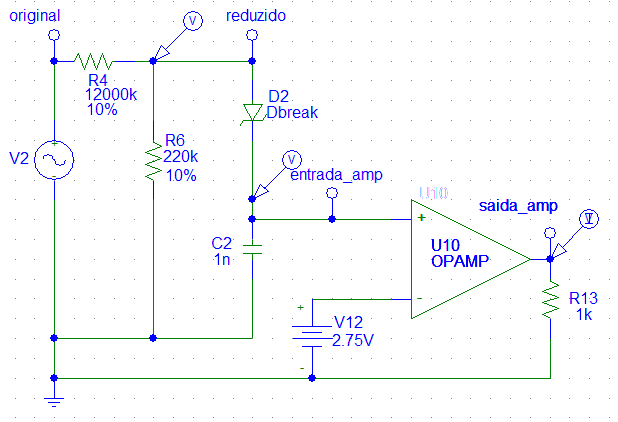
\includegraphics[width=9cm,keepaspectratio]{figuras/voltage-circuit.png}
\caption{\label{fig:voltage-circuit} Circuito verificador de tensão}
\end{figure}

\subsubsection{Medidor de Corrente}

Ainda no módulo sensor, é necessário obter as medidas do valor eficaz da corrente. O sensor não-invasivo produz uma tensão alternada na saída, e antes da coleta de dados pelo arduino é preciso obter um valor significativo, que não ultrapasse 2.5V. Para isso foi utilizado o circuito da figura \ref{fig:sensor-circuit}.

\begin{figure}[H]
\centering
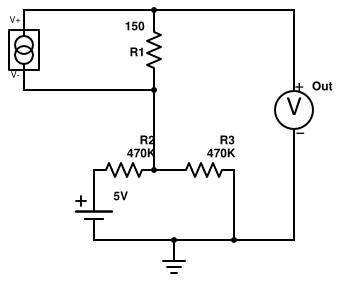
\includegraphics[width=9cm,keepaspectratio]{figuras/current-circuit.jpg}
\caption{\label{fig:sensor-circuit} Circuito medidor de corrente}
\end{figure}
%
\subsection{Peças}
\subsubsection{Sensor de Corrente Não-invasivo AC}

Esse sensor de corrente (figura \ref{fig:sensor}) consegue medir a corrente que passa por um fio de modo não-invasivo. O sensor é um transformador de corrente respondendo ao campo magnético formado em volta do fio condutor. Este, em particular, suporta até 30A de entrada, e necessita de um resistor de saída para obter a medida desejada em tensão \cite{non_invasive_sensor}.

\begin{figure}[H]
\begin{center}
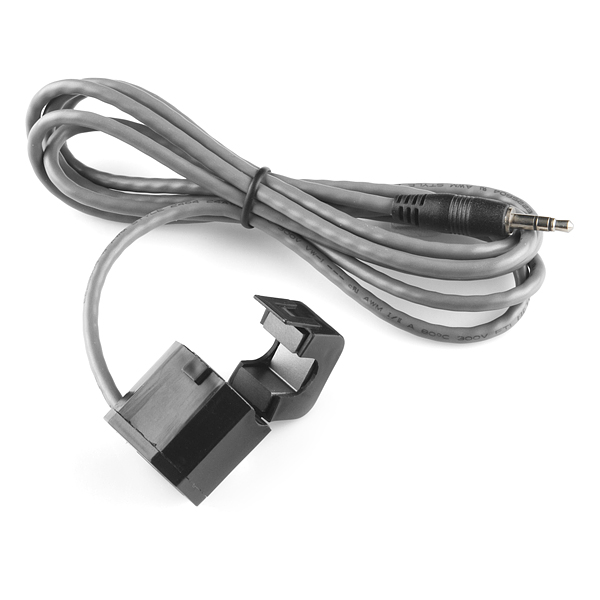
\includegraphics[width=5cm,height=5cm,keepaspectratio]{figuras/sensor.jpg}
\caption{\label{fig:sensor} Non-invasive AC current sensor}
\end{center}
\end{figure}

Algumas outras especificações são:
\begin{itemize}
\item{Corrente suportada: 30A}
\item{Temperatura de operação: -40$^{\circ}$C até 65 $^{\circ}$C}
\item{Precisão de 2\%}
\end{itemize}
%
\subsubsection{Raspberry Pi 2 modelo B}

A Raspberry Pi 2 Modelo B (figura \ref{fig:raspberry pi}) é o computador utilizado no sistema para receber os dados enviados pelos módulos sensores, tratá-los e enviá-los para a aplicação Web. Foi escolhido o Raspberry Pi por facilidade de projeto. Foi escolhido o modelo 2 - Model B por ser mais veloz, por possuir mais entradas USB e ser de alta disponibilidade no mercado, por um preço razoável. O kit inclui a fonte, um cartão microSD de 8GB e um adaptador Wifi USB. Mais detalhes estão no datasheet \cite{raspberry_datasheet}.

\begin{figure}[H]
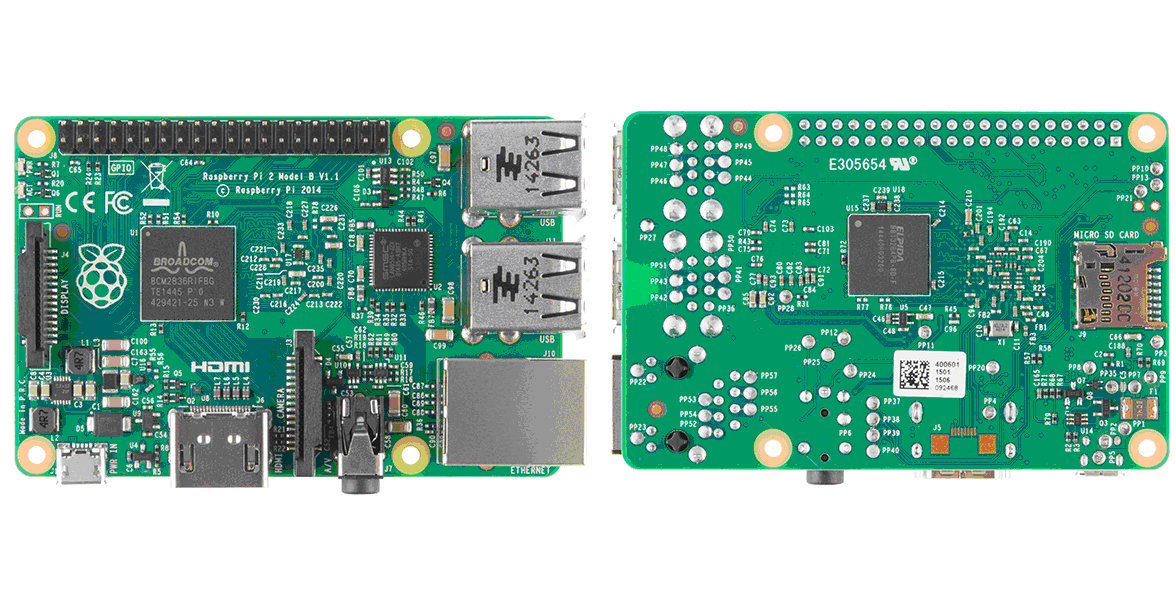
\includegraphics[width=1\textwidth]{figuras/raspberry_pi.png}
\caption{\label{fig:raspberry pi} Raspberry pi 2 modelo B}
\end{figure}

Especificações técnicas:
\begin{itemize}
\item{A 900MHz quad-core ARM Cortex-A7 CPU}
\item{1GB RAM}
\item{40 pinos GPIO}
\item{saída Full HDMI}
\item{porta Ethernet}
\item{entrada para cartão Micro SD}
\item{4 entradas USB}
\end{itemize}
%
\subsubsection{Arduino UNO}

Arduino \cite{arduino_site} é uma placa programável open-source. No projeto em questão esse componente receberá os dados do sensor, fará um tratamento e terá o envio programado desses para o coordenador. Pelo Arduino ser programável e possuir uma interface muito amigável, simplifica essa ponte entre a coleta de dados e a transmissão. E sua alta disponibilidade no mercado , assim como o raspberry, facilita sua obtenção. O modelo usado é o UNO (figura \ref{fig:arduino uno})

\begin{figure}[H]
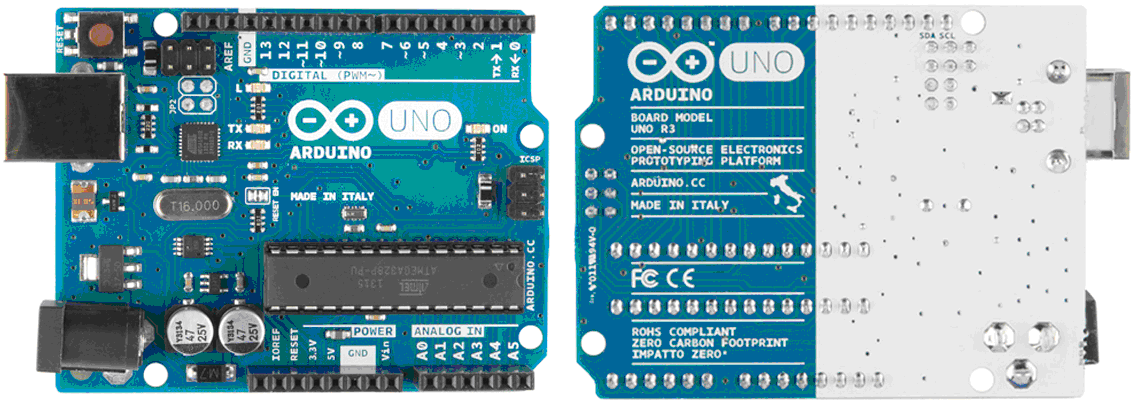
\includegraphics[width=1\textwidth]{figuras/arduino_uno.png}
\caption{\label{fig:arduino uno} Arduino UNO R3}
\end{figure}

Algumas outras especificações são:
\begin{itemize}
\item{microcontrolador ATmega328}
\item{tensão de entrada - 7-12V}
\item{14 Pinos Digital I/O (6 PWM de saída)}
\item{6 Inputs Analógicos}
\item{32k de memória Flash}
\item{16Mhz de Relógio}
\end{itemize}
%
\subsubsection{XBee}

É um módulo que permite uma comunicação simples e confiável entre microcontroladores, computadores, sistemas através de uma porta serial com um consumo menor de energia. Pode ser utilizado em redes ponto-a-ponto e multi-ponto. Foram escolhidos módulos da série 2 (figura \ref{fig:xbee}) por serem configuráveis através de um software da mesma empresa \cite{xctu_software}.

\begin{figure}[H]
\begin{center}
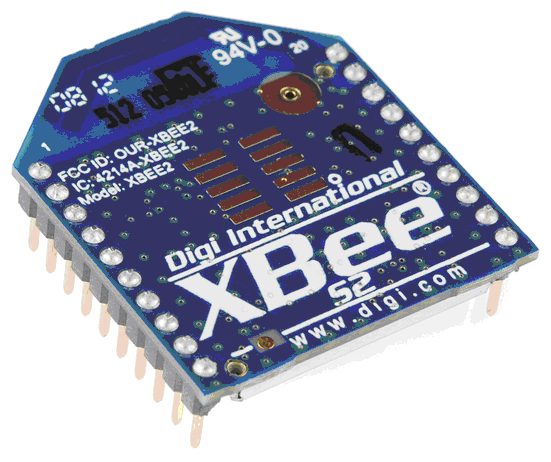
\includegraphics[width=5cm,height=5cm,keepaspectratio]{figuras/xbee_serie2.png}
\caption{\label{fig:xbee} XBee Serie 2}
\end{center}
\end{figure}

Algumas outras especificações são:
\begin{itemize}
\item{entradas de 3.3V @ 40mA}
\item{transmissão de dados máxima de 250kbps}
\item{potência de saída: 2mW (+3dBm)}
\item{alcance máximo de 120m}
\item{08 pinos digitais entrada/saída}
\item{encriptação 128-bit}
\item{configuração local ou remota}
\item{conector de antena RPSMA}
\end{itemize}
%
\subsubsection{XBee Explorer Dongle}

É um módulo com porta USB que faz a conexão do módulo XBee a um computador (figura \ref{fig:xbee explorer dongle}). Isso é necessário para ter acesso aos pinos de comunicação serial e de programação. Ele possui um conversor serial, que traduz os dados entre o computador e o XBee. Possui um botão de reset e um regulador de tensão para suprir a tensão necessária para XBee. Além disso possui 4 leds para debug: RX, TX, RSSI e indicador de energia. No projeto, este módulo é utilizado para fazer as configurações iniciais de todos os XBees e para conectar o XBee coordenador ao Raspberry Pi. Apesar de não ser um dispositivo essencial, este facilita muito nas tarefas citadas,  principalmente por lidar com a alimentação de 3,3V do XBee. Sendo um projeto aberto de hardware, seu desenho esquemático é acessível para uso público \cite{xbee_explorer_dongle_schematic}. 

\begin{figure}[H]
\begin{center}
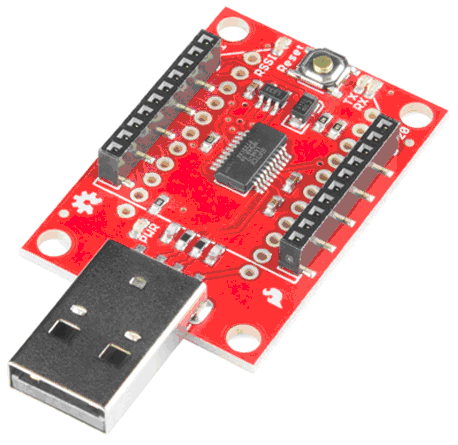
\includegraphics[width=5cm,height=5cm,keepaspectratio]{figuras/xbee_explorer_dongle.png}
\caption{\label{fig:xbee explorer dongle} XBee Explorer Dongle}
\end{center}
\end{figure}

\subsubsection{XBee Shield}

É um módulo que faz a conexão entre um módulo XBee e um Arduino (figura \ref{fig:xbee shield}). Ele possui opções para escolher se a conexão vai ser nos pinos UART ou qualquer outros pinos digitais do Arduino. A alimentação de 5V vinda do Arduino é regulada para 3.3V VDC antes de chegar no módulo XBee. O XBee Shield inclui LEDs para indicar a utilização dos pinos DIN, DOUT, RSSI e DIO5 do XBee. É usado um módulo XBee Shield para cada par XBee + Arduino. Assim como o XBee Explorer Dongle, seu esquemático também é acessível para uso público \cite{xbee_shield_schematic}. 

\begin{figure}[H]
\begin{center}
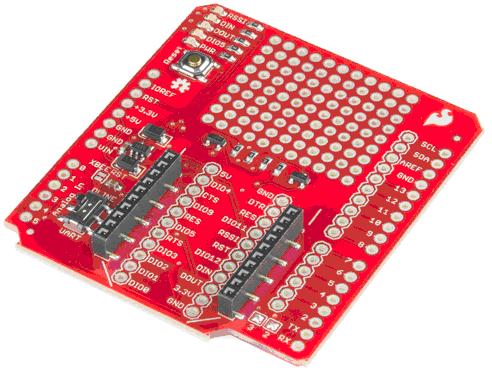
\includegraphics[width=5cm,height=5cm,keepaspectratio]{figuras/xbee_shield.png}
\caption{\label{fig:xbee shield} XBee shield do arduino UNO}
\end{center}
\end{figure}

\subsubsection{Arduino Stackable Header Kit - R3}

São conectores usados para encaixar o módulo XBee Shield no Arduino Uno R3 (figura \ref{fig:xbee shield headers}). Estão inclusos 4 headers, 2 x 8 pinos, 1 x 10 pinos e 1 x 6 pinos, suficientes para 1 módulo XBee Shield. Como há 2 sensores no projeto, serão usados 2 kits, com um adicional de reserva.

\begin{figure}[H]
\begin{center}
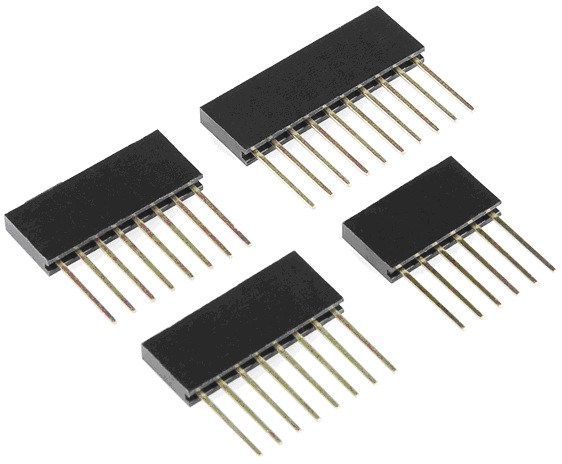
\includegraphics[width=5cm,height=5cm,keepaspectratio]{figuras/headers.png}
\caption{\label{fig:xbee shield headers} Headers usados no XBee shield}
\end{center}
\end{figure}


\section{Escopo}

Coletados os dados, resta mostrar informações úteis ao usuário. Com o consumo de corrente e a voltagem da tomada, é possível calcular a potência e alguns outros dados interessantes para o usuário. O aplicativo desenvolvido nesse trabalho é responsável por esse tratamento e a visualização dos dados coletados pelos sensores. As principais metas são as seguintes:

\begin{itemize}
	\item{informar ao usuário sobre o consumo de energia por equipamento em sua residência}
	\item{auxiliar o usuário a tomar decisões para diminuir o consumo de energia}
  \item{permitir o acesso às informações de consumo tanto localmente quanto remotamente}
\end{itemize}
%
\section{Funções do Sistema}

\begin{description}
	\item[Gerenciar contas:] O usuário poderá fazer cadastro/alteração de conta e autenticação.
	\item[Gerenciar equipamentos:] O usuário poderá fazer criação, edição e remoção de equipamentos, os quais serão monitorados pelo sistema
	\item[Gerenciar sensores:] Os módulos sensores são auto-detectados, e o usuário poderá editar ou removê-los
	\item[Gerenciar metas:] O usuário poderá criar, editar e remover metas mensais.
	\item[Gerenciar consumo:] O módulo coordenador enviará consumos para o sistema estes serão cadastrados. O usuário poderá visualizar os consumos através de gráficos. Além disso o usuário poderá importar ou exportar dados de consumo
	\item[Atualizar taxas da AES:] O usuário poderá atualizar as taxas de energia utilizadas para cálculo do custo do consumo
	\item[Configurar sistema:] O usuário poderá associar os sensores aos equipamentos e escolher um tipo de renda
\end{description}

\section{Requisitos não Funcionais}

\begin{itemize}
	\item{independência do usuário em relação ao técnico do sistema para instalar o sistema em sua residência}
	\item{sistema de fácil manuseio pelo usuário morador da residência}
	\item{característica portátil para os componentes físicos do sistema}
\end{itemize}

\section{Software}
\label{Sec:software}
Para que a aplicação Web possa receber os dados de consumo enviados pelo Módulo Coordenador, é necessário haver uma estrutura de rotas, métodos para lidar com objetos de classes, controladores e páginas de exibição para interagir com o usuário. Para isso, foi escolhida a arquitetura MVC, e um framework que consegue lidar com tal arquitetura. E para tornar a aplicação disponível para o acesso remoto através de smartphones, tablets e notebooks, optou-se por utilizar serviços de nuvem. 

\subsection{Tecnologia}

A seguir são apresentadas as tecnologias utilizadas para a implementação da aplicação Web.

\subsubsection{Django e Python}

O framework Django \cite{django_framework_site} foi utilizado devido ao uso da linguagem python, que é uma linguagem limpa, de fácil utilização e com ampla disponibilidade de bibliotecas gratuitas e de fóruns para auxílio na implementação. Uma das vantagens do python nesse caso é a compatibilidade, pois o hardware foi construído com intenção de aprendizado através da linguagem de programação python \cite{raspberry_pi_site}(``pi'' em ``raspberry pi'' vem de ``python''). Outra vantagem é a experiência dos integrantes do grupo quanto ao manuseio do framework, o que agilizou o desenvolvimento. Outra vantagem é a possibilidade de utilizar, se necessário, o próprio raspberry como servidor da aplicação, bastando instalar as bibliotecas das dependências do Django.

O Django utiliza a arquitetura MVC. Os Models no Django contém os campos e os métodos dos objetos sendo utilizados. Todos as classes de Models herdam métodos e atributos da classe pré-existente Model do Django. Geralmente, cada Model é mapeado para uma tabela no banco de dados.

As Views (na arquitetura MVC) são chamadas Templates no Django. Elas são páginas no formato HTML que podem conter trechos de código em python para mostrar conteúdo do Context. Context é uma estrutura de chave-valor que provê o conteúdo a ser utilizado na página.

Os Controllers são chamados Views. O Django provê os chamados Base Views, que são classes que auxiliam a criação de Controllers. Podem ser utilizados diretamente, sobrescrevendo seus atributos e métodos, ou herdando estes para classes customizadas. Há três Base Views: 
\begin{description}
	\item[View:] É a classe a partir da qual se herdam todas as outras classes de Controllers.
	\item[TemplateView:] Renderiza um Template com um Context.
	\item[RedirectView:] Redireciona para uma dada URL.
\end{description} 

Outros Controllers pré-existentes são os Generic Display Views, que são Controllers genéricos utilizados normalmente para exibir dados de Models:
\begin{description}
	\item[DetailView:] Exibe detalhes um objeto.
	\item[ListView:] Exibe uma lista de objetos.
\end{description}

Há Controllers utilizados para edição de conteúdo, que são os Generic Editing Views:
\begin{description}
	\item[FormView:] Exibe um formulário e realiza validação e redirecionamento caso não haja erros.
	\item[CreateView:] Exibe um formulário para criação de objetos. Caso o formulário seja submetido e não haja erros na validação, cria o objeto.
	\item[UpdateView:] Exibe um formulário para edição de objetos. Caso o formulário seja submetido e não haja erros na validação, salva o objeto.
	\item[DeleteView:] Exibe uma página com uma caixa de confirmação para deletar um objeto.
\end{description}

\subsubsection{Heroku}

Heroku é uma plataforma em nuvem que fornece múltiplos serviços para dar suporte a uma aplicação web. É possível hospedar aplicações em linguagens como Node, Ruby, Java, PHP, Python, Go, Scala, ou Clojure, e o Heroku a manterá no ar sem a necessidade da intervenção do desenvolvedor. Esse serviço, diferente de opções de outros serviços de nuvem como o da Amazon, se encarrega em configurar o ambiente de execução da aplicação, o que agiliza o processo de colocar a aplicação em produção.

Heroku utiliza os chamados dynos, que representam máquinas/computadores que executam comandos. Cada tipo de dyno possui a sua limitação de memória RAM, fração de CPU, se é dedicada ou não e a velocidade do processamento, que refletem nos custos de aquisição dos serviços, porém, existe a opção gratuita que permite colocar uma aplicação em produção com um processamento suficiente para atender tráfegos pequenos. Nos planos pagos, o sistema é escalável (pode-se alterar o limite do número de processos em execução na máquina do sistema, memória RAM, entre outros) para atender a momentos de tráfego mais intenso.\cite{heroku}

Durante a fase de teste do sistema em questão é utilizado o plano gratuito do Heroku.

\subsection{Funções do Sistema}

A aplicação Web possui tem como objetivo mostrar os dados de consumo para o usuário, mas a aplicação deve possuir outras funções para alcançar o objetivo. Uma delas é criar uma conta. Para que o usuário possa manter seus dados confidenciais, a aplicação permite autenticação através de senha e nome de usuário. Equipamentos são  representados dentro do sistema, para que cada consumo possa se associar a um equipamento, e para isso, é necessário que o usuário gerencie os seus equipamentos. Os sensores também são representados dentro do sistema, pois um usuário tem a opção de alocar o sensor de um equipamento para outro, caso deseje. O Módulo Coordenador cria os consumos dentro do sistema, enquanto o usuário visualiza, importa e exporta os consumos. Para que a conversão do consumo em unidades monetárias seja possível, o usuário deve atualizar as taxas da AES dentro do sistema. E para fazer a associação entre um sensor e um equipamento e atualizar suas informações de renda, o usuário deve configurar o sistema. A partir dessas informações foi criada a seguinte lista de funções para a aplicação:

\begin{description}
	\item[Gerenciar contas:] O usuário pode fazer cadastro/alteração de conta e autenticação.
	\item[Gerenciar equipamentos:] O usuário pode fazer a criação, edição e remoção de equipamentos.
	\item[Gerenciar sensores:] Os módulos sensores são auto-detectados, e o usuário pode editá-los ou removê-los.
	\item[Gerenciar metas:] O usuário pode criar, editar e remover metas mensais.
	\item[Gerenciar consumo:] O Módulo Coordenador envia consumos para o sistema. O usuário pode visualizar os consumos através de gráficos. Além disso o usuário pode importar ou exportar dados de consumo.
	\item[Atualizar taxas da AES:] O usuário pode atualizar as taxas de energia utilizadas para cálculo do custo do consumo.
	\item[Configurar sistema:] O usuário pode associar os sensores aos equipamentos e escolher um tipo de renda.
\end{description}

\subsection{Atores}

A partir da descrição dos casos de uso (apêndice \ref{apendice_caso_uso}), dois atores foram identificados: o usuário e o módulo coordenador, que são as entidades externas que interagem com o sistema.

\begin{description}
	\item[usuário:] Como o sistema vai ser utilizado apenas pelo(s) responsável(is) pela residência, há apenas um tipo de usuário, que é o usuário comum.
    \item[módulo coordenador:] É o componente de hardware que enviará informações de consumo para o sistema
\end{description}

%
\subsection{Classes e atributos}

A partir dos casos de uso foi possível a identificação das classes dentro do sistema: Equipment, Consumption, Sensor, AESRate, Goal, User. Essas classes e suas relações estão representadas pelo diagrama de classes na figura \ref{fig:diagrama-classes}.

\begin{figure}[H]
\begin{center}
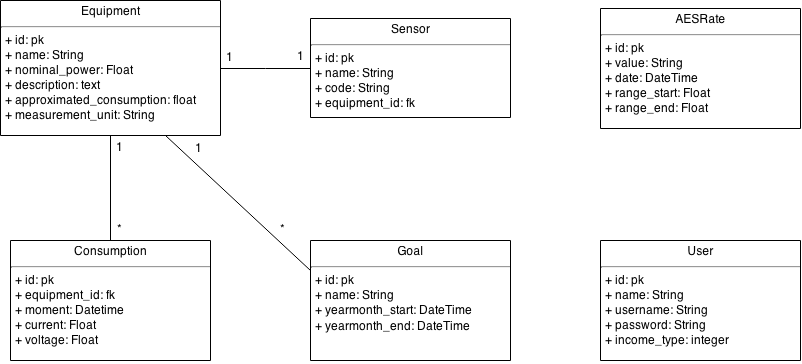
\includegraphics[width=1\textwidth]{figuras/diagrama_classes.png}
\caption{\label{fig:diagrama-classes} Diagrama de Classes}
\end{center}
\end{figure}

A descrição das classes está no apêndice \ref{apendice_classes}

\begin{figure}
\centering
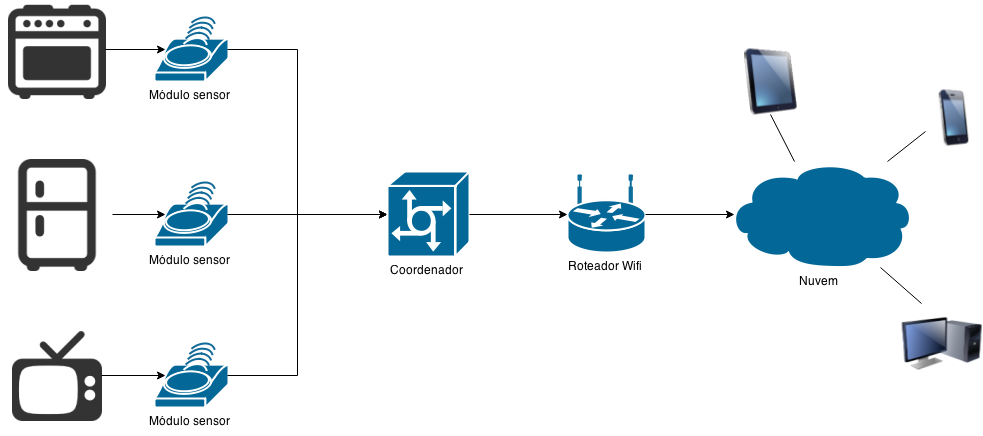
\includegraphics[width=1\textwidth]{figuras/esqueminha.png}
\caption{\label{fig:esqueminha} Esquema do Projeto}
\end{figure}

\begin{figure}
\centering
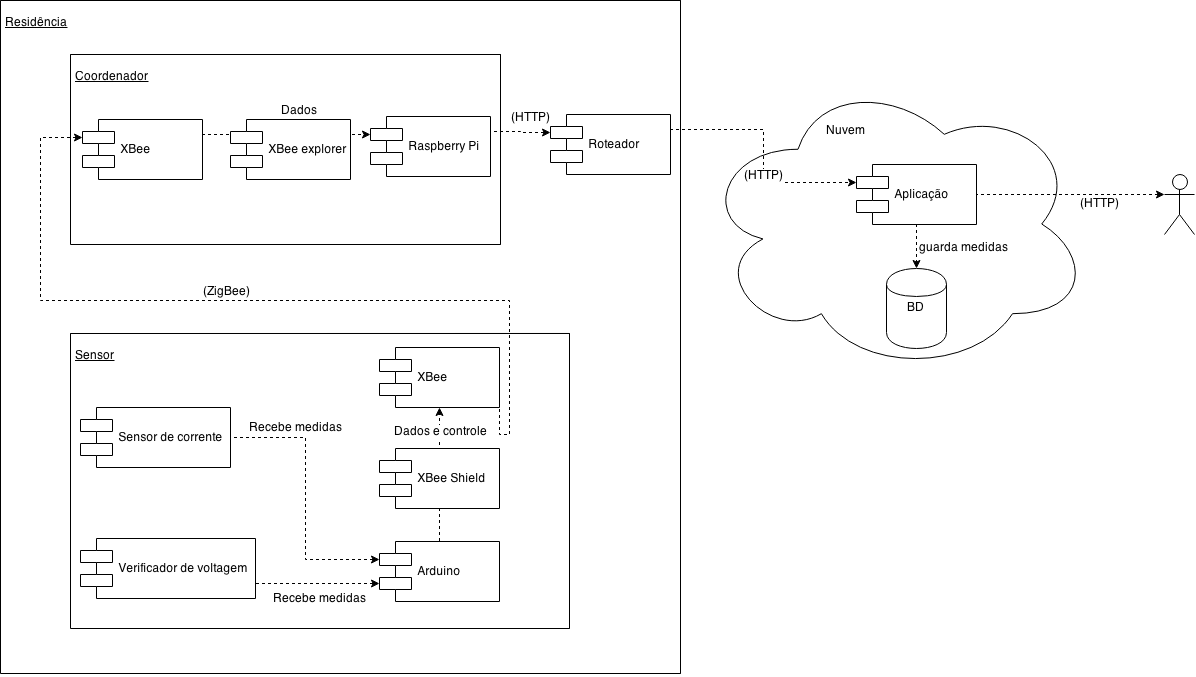
\includegraphics[width=1\textwidth]{figuras/diagrama_implantacao.png}
\caption{\label{fig:diagrama_implantacao} Diagrama de implantação}
\end{figure}
